\documentclass{article}
\usepackage{enumerate}
\usepackage{amsmath}
\usepackage{amssymb}
\usepackage{graphicx}
\usepackage{subfigure}
\usepackage{geometry}
\usepackage{caption}
\usepackage{indentfirst}

\usepackage{algorithm}
\usepackage{algorithmicx}
\usepackage{algpseudocode}
\renewcommand{\algorithmicrequire}{\textbf{Input:}}
\renewcommand{\algorithmicensure}{\textbf{Output:}}

\geometry{left=3.0cm,right=3.0cm,top=3.0cm,bottom=4.0cm}
\renewcommand{\thesection}{Exercise 7.\arabic{section}}
\title{VE203 Assignment 7}
\author{Liu Yihao 515370910207}
\date{}
\begin{document}
\maketitle

\section{}
\begin{enumerate}[i)]
\item
Use full line to express two people are friends and dotted line to express two people are enemies, we get Figure \ref{e1_1}. So it is proved.

\begin{figure}[H]
	\centering
	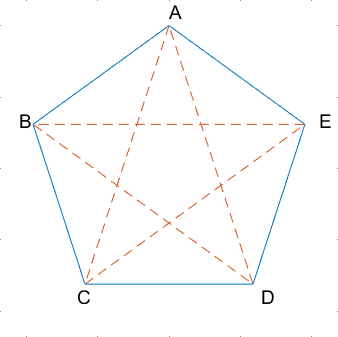
\includegraphics[scale=0.4]{e1_1.png}
	\caption{The relationship between five people.}
	\label{e1_1}
\end{figure}

\item
Consider one member of the group, A. The nine other numbers of the party are either friends or enemies of A. By the generalized pigeonhole principle, at least five of them are either friends or enemies of A. Suppose that B, C, D, E, F are friends of A. If any two of these three are friends, then they together with A are a group of three mutual friends. If none of B, C, D, E, F are friends, then they form a group of four mutual enemies. Vice versa, there are either three mutual enemies and four mutual friends.

\item
Consider one member of the group, A. The nineteen other numbers of the party are either friends or enemies of A. By the generalized pigeonhole principle, at least ten of them are either friends or enemies of A. Suppose that they are friends of A. If there are three mutual friends in these ten people, then they together with A are a group of four mutual friends. If there are four mutual enemies, then they form a group of four mutual enemies. Then suppose ten of them are enemies of A. If there are three mutual enemies in these ten people, then they together with A are a group of four mutual enemies. If there are four mutual friends, then they form a group of four mutual friends.

\item
We need to prove that in a group of $n$ people, there are either two mutual friends or $n$ mutual enemies. If any two of these $n$ are friends, then there are two mutual friends. Otherwise, if all of the people are enemies, then there are $n$ mutual enemies. So it is proved.

\item
We need to prove that in a group of $R(m-1,n)+R(m,n-1)$ people, there are either $m$ mutual friends or $n$ mutual enemies. Consider one member of the group, A. The $R(m-1,n)+R(m,n-1)-1$ other numbers of the party are either friends or enemies of A. Suppose $R(m-1,n)\leqslant R(m,n-1)$, and the generalized pigeonhole principle, at least $R(m-1,n)$ of them are either friends or enemies of A. Suppose they are friends of A. If any $m-1$ of these $R(m-1,n)$ are friends, then they together with A are a group of $m$ mutual friends. If $n$ of these $R(m-1,n)$ are friends, then they form a group of $n$ mutual enemies. Then suppose $R(m-1,n)$ of them are enemies of A, and $R(m-1,n)=R(n,m-1)$, so we can simply conclude the same result as above. Then the statement is proved.\\
$R(4,3)\leqslant R(3,3)+R(4,2)=10$

\item
Consider first the case where there is one person with four or more friends. Then if any two of these four are friends, then they together with the person are a group of three mutual friends. If none of these four are friends, then they form a group of four mutual enemies.\\
Consider secondly the case where no one has four or more friends, i.e., everyone has five or more enemies. Then at most four of these five are mutual friends since no one has four or more friends, so at least two of these five are mutual enemies,  then they together with the person are a group of three mutual enemies.

\item
Use full line to express two people are friends and dotted line to express two people are enemies, we get Figure \ref{e1_7}. So it is proved.

\begin{figure}[H]
	\centering
	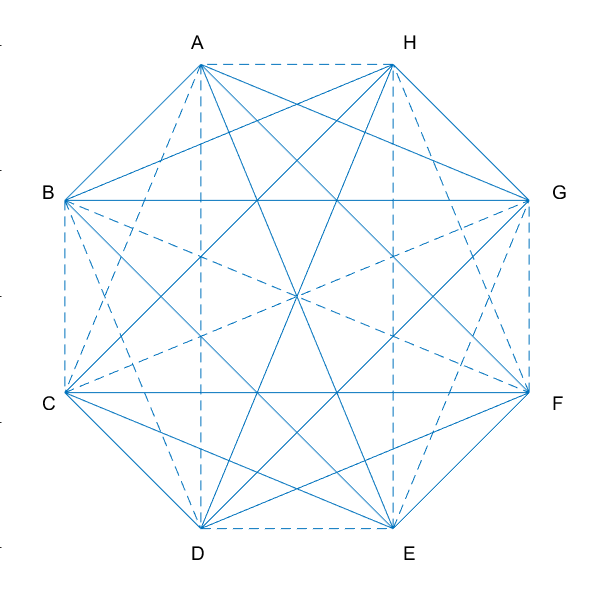
\includegraphics[scale=0.4]{e1_7.png}
	\caption{The relationship between eight people.}
	\label{e1_7}
\end{figure}

Since $R(4,3)>8$ and $R(4,3)\leqslant 9$, $R(4,3)=9$

\end{enumerate}

\section{}
Suppose there are $n$ people, and there aren't two people at the party who have the same number of friends, then all people at the party have different number of friends. So there is one people having no friend and one people having all of $n-1$ friends, which reaches a contradiction. So it is proved.

\section{}
We need to show
\begin{equation*}
\left(\begin{array}{l}n\\k\\\end{array}\right)
=\frac{1}{k!}\cdot\frac{n!}{(n-k)!}\leqslant\frac{n^k}{2^{k-1}}
\end{equation*}

Firstly, we show $k!\geqslant 2^{k-1}$\\
\indent
For $k=0$, $1=k!>2^{k-1}=0$, for $k=1$, $k!=2^{k-1}=1$\\
\indent
For $k=m,m\in N^+$, suppose $m!\geqslant 2^{m-1}$ is true\\
\indent
Then for $k=m+1$, $(m+1)!=(m+1)m!$, $2^m=2\cdot2^{m-1}$. Since $m+1\geqslant 2$, it is also true.\\
\indent
So $k!\geqslant 2^{k-1}$ is proved\\

Secondly, we show $\dfrac{n!}{(n-k)!}\leqslant n^k$
$$\frac{n!}{(n-k)!}=\prod_{i=1}^{k} n-k+i$$
$$n^k=\prod_{i=1}^{k} n$$

Since $-k+i\leqslant 0$, each item of $\dfrac{n!}{(n-k)!}\leqslant n^k$, so it is proved.\\

In conclusion, since the two inequalities form, it is proved.

\section{}

According to theorem 2.5.1,
$$P[A\cup B]=P[A]+P[B]-P[A\cap B]$$

Since $P[A\cap B]<=1$, we get
$$P[A\cup B]\geqslant P[A]+P[B]-1$$

\section{}

For $n=1$, $P[A_1]=P[A_1]$, so it is true.\\
\indent
For $n=m,m\in N^+$, suppose it is true.\\
\indent
Then for $n=m+1$, according to theorem 2.5.1,\\

\begin{align*}
P[A_1\cup A_2\cup\cdots\cup A_{m+1}]
&=P[A_1\cup A_2\cup\cdots\cup A_m]+P[A_{m+1}]-P[(A_1\cup A_2\cup\cdots\cup A_m)\cap A_{m+1}]\\
&=P[A_1\cup A_2\cup\cdots\cup A_m]+P[A_{m+1}]-P[(A_1\cup A_2\cup\cdots\cup A_{m-1})\cap A_{m+1}]\\
&\quad-P[A_m\cap A_{m+1}]+P[(A_1\cup A_2\cup\cdots\cup A_{m-1})\cap A_m\cap A_{m+1}]\\
&=\cdots\\
&=\sum_{1\leqslant i\leqslant m}P[A_i]+P[A_{m+1}]-\sum_{1\leqslant i<j\leqslant m}P[A_i\cap A_j]-\sum_{1\leqslant i\leqslant m-1}P[A_i\cap A_{m+1}]\\
&\quad-P[A_m\cap A_{m+1}]+\sum_{1\leqslant i<j<k\leqslant m}P[A_i\cap A_j\cap A_k]+\sum_{1\leqslant i\leqslant m-2}P[A_i\cap A_{m}\cap A_{m+1}]\\
&\quad+P[A_{m-1}\cap A_{m}\cap A_{m+1}]-\cdots+\cdots+(-1)^{m+2}P[A_1\cap A_2\cap\cdots\cap A_{m+1}]\\
&=\sum_{1\leqslant i\leqslant m+1}P[A_i]-\sum_{1\leqslant i<j\leqslant m+1}P[A_i\cap A_j]+\sum_{1\leqslant i<j<k\leqslant m+1}P[A_i\cap A_j\cap A_k]\\
&\quad-\cdots+\cdots+(-1)^{m+2}P[A_1\cap A_2\cap\cdots\cap A_{m+1}]
\end{align*}


\section{}
\begin{algorithm}
\begin{algorithmic}[1]
	\Require $L=\langle l_1,\cdots,l_n \rangle$, a list of n elements, the number of steps $k$
	\Ensure If the list is not sorted, return $true$, else, return $false$
	\Function{unsorted}{$L,n,k$}
		\If{$k \geqslant n$}
			\State $k \gets n-1$
		\EndIf
		\For{$i \gets 1$ \textbf{to} $k$}
    		\State $r \gets rand(n-1)$
    		\If{$l_{r+1}<l_r$}
    			\State \Return $true$
    		\EndIf
    		\State \textbf{Remove} $l_r$ \textbf{from} $L$
    		 \State $n \gets n-1$
    	\EndFor
    	\State \Return $false$
    \EndFunction
\end{algorithmic}
\end{algorithm}

Since probability to be correct is $n-1$ choose $k$, the incorrect probability can be expressed as
\begin{equation*}                         
P=\left\lbrace
\begin{array}{ll}
\dfrac{k!}{(n-1)!}&k<n\\
0&k\geqslant n\\
\end{array}
\right.
\end{equation*}

\section{}
\begin{enumerate}[i)]
\item
If $n$ is prime and $b\in N\backslash\lbrace0\rbrace$ with $b\nmid n$, we can use Fermat's Little Theorem to get
$$b^{n-1}\equiv 1{\rm \ (mod\ }n)$$
Since $t=\dfrac{n-1}{2^s}\in N$,
$$b^{2^{s-1}t}=b^{\frac{n-1}{2}}\equiv \pm 1{\rm \ (mod\ }n)$$
which means
$$b^{2^{s-1}t}=b^{\frac{n-1}{2}}\equiv -1{\rm \ (mod\ }n)$$
or
$$b^{2^{s-1}t}=b^{\frac{n-1}{2}}\equiv 1{\rm \ (mod\ }n)$$
The first situation satisfy the definition, and the second situation can be deduced again to
$$b^{2^{s-2}t}=b^{\frac{n-1}{4}}\equiv \pm 1{\rm \ (mod\ }n)$$
Repeat this procedure, we can get
$$b^{2^{j}t}=b^{\frac{n-1}{2^{s-j}}}\equiv -1{\rm \ (mod\ }n),j\in[0,s-1],j\in N$$
or
$$b^{t}=b^{\frac{n-1}{2^s}}\equiv 1{\rm \ (mod\ }n)$$
\item
We need to find
$$2^t=2^{\frac{2047-1}{2^s}}\equiv 1{\rm \ (mod\ }2047)$$
When $s=1$, it can be deduced to
$$2^t=2^{1023}\equiv \pm 1{\rm \ (mod\ }2047)$$
Since $1023=11\times93$ and $2^{11}\equiv 1{\rm \ (mod\ }2047)$
$$2^{1023}=2^{11\times93}\equiv 1{\rm \ (mod\ }2047)$$
So 2047 passes Miller's test to the base 2, but $2047=23\times89$, it is composite.
\end{enumerate}


\end{document}
